\documentclass{article}
\usepackage{spikey}
\usepackage{amsmath}
\usepackage{mathrsfs}
\usepackage{amssymb}
\usepackage{soul}
\usepackage{float}
\usepackage{graphicx}
\usepackage{hyperref}
\usepackage{fancyhdr}
\usepackage{xcolor}
\usepackage{chngcntr}
\usepackage{centernot}
\usepackage[shortlabels]{enumitem}
\usepackage[margin=1truein]{geometry}
\usepackage{tkz-graph}
\usepackage{dsfont}
\usepackage{caption}
\usepackage{subcaption}
\usepackage[yyyymmdd,hhmmss]{datetime}

\usepackage{setspace}
\linespread{1.15}
\usepackage[margin=1truein]{geometry}

\counterwithin{equation}{section}
\counterwithin{figure}{section}

\usepackage{listings}
 
\definecolor{codegreen}{rgb}{0,0.6,0}
\definecolor{codegray}{rgb}{0.5,0.5,0.5}
\definecolor{codeblue}{rgb}{0.3,0.5,0.8}
\definecolor{codepurple}{rgb}{0.58,0,0.82}
%\definecolor{backcolour}{rgb}{0.95,0.95,0.92}
\definecolor{backcolour}{rgb}{1,1,1}

\lstdefinestyle{mystyle}{
    backgroundcolor=\color{backcolour},   
    commentstyle=\color{codegreen},
    keywordstyle=\color{magenta},
    numberstyle=\tiny\color{codegray},
    stringstyle=\color{codepurple},
    basicstyle=\ttfamily\footnotesize,
    breakatwhitespace=false,         
    breaklines=true,                 
    captionpos=b,                    
    keepspaces=true,                 
    numbers=left,                    
    numbersep=5pt,                  
    showspaces=false,                
    showstringspaces=false,
    showtabs=false,                  
    tabsize=4
}

\lstset{style=mystyle}

\title{CSC413: Homework 1}
\date{\today\ at \currenttime}
\author{Tianyu Du (1003801647)}
\begin{document}
    \maketitle
    \section{Hard-Coding Networks}
    \subsection{Verify Sort}
    \begin{proof}[Soln]
    	The first layer performs pairwise comparison to construct indicators $\id{x_1 \leq x_2}$, $\id{x_2 \leq x_3}$, and $\id{x_3 \leq x_4}$. The second layer performs an \texttt{all()} operation on indicators from the previous layer.
    	\begin{align}
    		\textbf{W}^{(1)} = 
    		\begin{pmatrix}
    			-1 & 1 & 0 & 0 \\
    			0 & -1 & 1 & 0 \\
    			0 & 0 & -1 & 1
    		\end{pmatrix}
    	\end{align}
    	\begin{align}
    		\textbf{b}^{(1)} = 
    		\begin{pmatrix}
    			0 & 0 & 0
    		\end{pmatrix}
    	\end{align}
    	So that 
    	\begin{align}
    		\varphi(\textbf{h}) = \varphi(\textbf{W}^{(1)} \vex + \textbf{b}^{(1)}) =
    		\varphi \begin{pmatrix}
    			x_2 - x_1 \\
    			x_3 - x_2 \\
    			x_4 - x_3
    		\end{pmatrix} =
    		\begin{pmatrix}
    			\id{x_2 \geq x_1} \\
    			\id{x_3 \geq x_2} \\
    			\id{x_4 \geq x_3}
    		\end{pmatrix}
    	\end{align}
    	\begin{align}
    		\textbf{w}^{(2)} = 
    		\begin{pmatrix}
    			1 & 1 & 1
    		\end{pmatrix}
    	\end{align}
    	\begin{align}
    		b^{(2)} = - 2.5
    	\end{align}
    	Such that $y = 1$ if and only if all components of \textbf{h} are ones, i.e., the list is sorted.
    \end{proof}

	\subsection{Perform Sort}
	\begin{proof}
		For this section, I am implementing a feedforward neural network performing bubble sort. \\
		Note that given $\vex = (x_1, x_2, x_3, x_4)$, the \textbf{swapping} operation can be conducted by multiplying $\vex$ by a matrix. \\
		For instance, the following $\textbf{W}^{(12)}$ swaps the first and second elements.
		\begin{align}
			\underbrace{\begin{pmatrix}
				0 & 1 & 0 & 0 \\
				1 & 0 & 0 & 0 \\
				0 & 0 & 1 & 0 \\
				0 & 0 & 0 & 1
			\end{pmatrix}}_{\textbf{W}^{(12)}} (x_1, x_2, x_3, x_4)^T
			&= (x_2, x_1, x_3, x_4)^T
		\end{align}
		Let $\textbf{I}_4$ denote the identity matrix. Define the following neural network:
		\begin{align}
			\textbf{h}_1 &:= \id{x_1 \leq x_2} \textbf{I}_4 \vex
			+ \id{x_1 > x_2} \textbf{W}^{(12)} \vex \\
			\textbf{h}_2 &= \id{x_2 \leq x_3} \textbf{I}_4 \textbf{h}_1
			+ \id{x_2 > x_3} \textbf{W}^{(23)} \textbf{h}_1 \\
			\textbf{h}_3 &= \id{x_3 \leq x_4} \textbf{I}_4 \textbf{h}_2
			+ \id{x_3 > x_4} \textbf{W}^{(34)} \textbf{h}_2 \\
			\textbf{h}_4 &= \id{x_1 \leq x_2} \textbf{I}_4 \textbf{h}_3
			+ \id{x_1 > x_2} \textbf{W}^{(12)} \textbf{h}_3 \\
			\textbf{h}_5 &= \id{x_2 \leq x_3} \textbf{I}_4 \textbf{h}_4
			+ \id{x_2 > x_3} \textbf{W}^{(23)} \textbf{h}_4 \\
			\textbf{y}(\vex) &= \id{x_1 \leq x_2} \textbf{I}_4 \textbf{h}_5
			+ \id{x_1 > x_2} \textbf{W}^{(12)} \textbf{h}_5
		\end{align}
		The above neural network can also be implemented using a recurrent structure, in which hidden states record the number of pairwise comparisons made.9
	\end{proof}
	
	\subsection{Universal Approximation Theorem}
	\subsubsection{}
	\begin{proof}[Soln]
		To avoid over-using of notations, let $\varphi(y) := \id{y \geq 0}$ denote the activation function.
		\begin{align}
			n &= 2 \\
			\textbf{W}_0 &= (1, -1) \\
			\textbf{b}_0 &= (-a, b) \\
			\textbf{W}_1 &= (h, h) \\
			\textbf{b}_1 &= - h
		\end{align}
		Justification:
		\begin{align}
			\varphi(\textbf{h}) &= \varphi((x - a, b - x)) \\
			&= (\id{x-a \geq 0}, \id{b-x \geq 0}) \\
			&= (\id{x \geq a}, \id{x \leq b}) \\
			\textbf{W}_1 \varphi(\textbf{h}) + \textbf{b}_1
			&=\id{x \geq a} h + \id{x \leq b} h - h \\
			&=\id{a \leq x \leq b} h
		\end{align}
	\end{proof}
	\subsubsection{}
	\begin{proof}[Soln]
		Let $\delta \in (0, 1)$ denote the ratio parameter, a higher value of $\delta$ results in a finer approximation is. In this example, take $\delta = \frac{9}{10}$. \\
		Without loss of generality, assume the region $I$ on which function $f$ is defined on to be symmetric across zero. \\
		Let $I = [-1, 1]$, given $f$ is symmetric, $f(-\delta) = f(\delta)$. \\
		Define:
		\begin{align}
			\hat{f}_1(x) = \hat{f}_0(x) + g(
				f(\delta), -\delta, \delta, x
			)
		\end{align}
		Note that
		\begin{align}
			\norm{f - \hat{f}_1}
			&= \int_{-1}^1 \abs{f(x) - \hat{f}_1(x)}\ dx \\
			&= \int_{-1}^{-\delta} \abs{f(x)}\ dx
			+ \int_{-\delta}^\delta \abs{f(x) - \hat{f}_1(x)}\ dx
			+ \int_{\delta}^{1} \abs{f(x)}\ dx
		\end{align}
		Given that $\forall x \in (-\delta, \delta),\ f(x) > f(-\delta) = f(\delta) > 0$, it follows
		\begin{align}
			\int_{-\delta}^\delta \abs{f(x) - \hat{f}_1(x)}\ dx
			&= \int_{-\delta}^\delta f(x) - \hat{f}_1(x)\ dx \\
			&= \int_{-\delta}^\delta f(x)\ dx - \int_{-\delta}^\delta \hat{f}_1(x)\ dx
		\end{align}
		Also, $\int_{-\delta}^\delta \hat{f}_1(x)\ dx > 0$ provided $\delta \neq 0$. Therefore,
		\begin{align}
			\int_{-\delta}^\delta \abs{f(x) - \hat{f}_1(x)}\ dx &< \int_{-\delta}^\delta f(x)\ dx \\
			&= \int_{-\delta}^\delta \abs{f(x)}\ dx
		\end{align}
		Therefore,
		\begin{align}
			\norm{f - \hat{f}_1} &= \int_{-1}^{-\delta} \abs{f(x)}\ dx
			+ \int_{-\delta}^\delta \abs{f(x) - \hat{f}_1(x)}\ dx
			+ \int_{\delta}^{1} \abs{f(x)}\ dx \\
			&< \int_{-1}^{-\delta} \abs{f(x)}\ dx
			+ \int_{-\delta}^\delta \abs{f(x)}\ dx
			+ \int_{\delta}^{1} \abs{f(x)}\ dx \\
			&= \int_{-1}^1 \abs{f(x) - 0}\ dx \\
			&= \int_{-1}^1 \abs{f(x) - \hat{f}_0(x)}\ dx \\
			&= \norm{f(x) - \hat{f}_0(x)}
		\end{align}
		Therefore, 
		\begin{align}
			\norm{f(x) - \hat{f}_1(x)} &< \norm{f(x) - \hat{f}_0(x)}
		\end{align}
		\begin{figure}[H]
			\center
			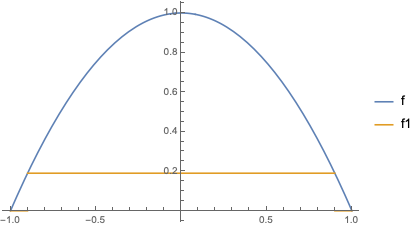
\includegraphics[width=0.7\linewidth]{plot_132.png}
			\caption{Approximated Result}
		\end{figure}
	\end{proof}
	\subsubsection{}
	\begin{proof}[Soln]
		\textbf{Algorithm:}
		\begin{enumerate}[(i)]
			\item Divide $I = [-1, 1]$ into $N+2$ sub-intervals with equal length, such that
			\begin{align}
				I_i := \left[
				-1 + \frac{i}{N+2},
				-1 + \frac{i+1}{N+2}
				\right]\quad \forall\ i \in \{1, 2, \cdots, N\}
			\end{align}
			Note that the first and last sub-intervals are not used to construct $g_i$.
			\item For each $i$, define
			\begin{align}
				h_i &:=\min_{x \in I_i} f(x) \\
				a_i &:= -1 + \frac{i}{N+2} \\
				b_i &:= -1 + \frac{i+1}{N+2}
			\end{align}
		\end{enumerate}
		Because $f(x) \geq 0\ \forall x \in I$.\\
		By the definition of $g_i(x)$, it can be shown that\footnote{I am excluding those boundary points between consecutive sub-intervals, because at those points, the value of $f_i$ spikes due to duplicate counts of indicator functions. However, while doing integral, this does not matter as the set of boundary points has measure zero.}
		\begin{align}
			f(x) \geq f_i(x)\ \forall i \in \{1, 2, \cdots, N\}\ \forall x \in \bigcup_{i=1}^N (a_i, b_i)
		\end{align}
		Further,
		\begin{align}
			f(x) = f_i(x)\quad \forall i \in \{1, 2, \cdots, N\}\ \forall x \in \left[-1, -1 + \frac{1}{N+2} \right) \bigcup \left (
			1 - \frac{1}{N+2}, 1 \right]
		\end{align}
		Define
		\begin{align}
			\mc{K} := \left[-1, -1 + \frac{1}{N+2} \right) \bigcup \left (
			1 - \frac{1}{N+2}, 1 \right] \bigcup \left(\bigcup_{i=1}^N (a_i, b_i) \right)
		\end{align}
		Note that the set $I \backslash \mc{K}$ consists of all boundary points between consecutive sub-intervals. There are only finitely many such points, therefore $I \backslash \mc{K}$ has measure zero, and
		\begin{align}
			\int_I \abs{f(x) - \hat{f}_i(x)}\ dx = \int_\mc{K} \abs{f(x) - \hat{f}_i(x)}\ dx
		\end{align}
		And I've shown that for every $i$ and every $x \in \mc{K}$, $f(x) \geq f_i(x)$. Consequently,
		\begin{align}
			\int_I \abs{f(x) - \hat{f}_i(x)}\ dx 
			&= \int_\mc{K} \abs{f(x) - \hat{f}_i(x)}\ dx \tx{ (removing measure zero set.)} \\
			&= \int_\mc{K} f(x) - \hat{f}_i(x)\ dx \\
			&= \int_I f(x) - \hat{f}_i(x)\ dx \tx{ (adding back the measure zero set.)}\quad (\dagger)
		\end{align}
		
		Define $\hat{f}_0(x) = 0$ and let $i \in \{1, 2, \cdots, N\}$,
		\begin{align}
			\norm{f - \hat{f}_{i+1}}
			&= \int_{-1}^1 \abs{f(x) - \hat{f}_{i+1}(x)}\ dx \\
			&= \int_{-1}^1 f(x) - \hat{f}_{i+1}(x)\ dx \tx{ by }(\dagger)\\
			&= \int_{-1}^{-1 \frac{i+1}{N}} f(x) - \hat{f}_{i+1}(x)\ dx 
			+ \int_{-1+\frac{i+1}{N}}^{-1+\frac{i+2}{N}} f(x) - \hat{f}_{i+1}(x)\ dx 
			+ \int_{-1+\frac{i+2}{N}}^1 f(x) - \hat{f}_{i+1}(x)\ dx
		\end{align}
		Further, by construction, $\hat{f}_{i+1}(x) = \hat{f}_i(x)\ \forall x \notin [a_{i+1}, b_{i+1}]$. Therefore,
		\begin{align}
			\norm{f - \hat{f}_{i+1}}
			&= \int_{-1}^{a_{i+1}} f(x) - \hat{f}_i(x)\ dx 
			+ \int_{a_{i+1}}^{b_{i+1}} f(x) - \hat{f}_{i+1}(x)\ dx 
			+ \int_{b_{i+1}}^1 f(x) - \hat{f}_i(x)\ dx \\
			&= \int_{-1}^{a_{i+1}} f(x) - \hat{f}_i(x)\ dx 
			+ \int_{a_{i+1}}^{b_{i+1}} f(x) - \hat{f}_{i}(x) - g(h_{i+1}, a_{i+1}, b_{i+1}, x)\ dx 
			+ \int_{b_i}^1 f(x) - \hat{f}_i(x)\ dx \\
			&= \int_{-1}^{a_{i+1}} f(x) - \hat{f}_i(x)\ dx 
			+ \int_{a_{i+1}}^{b_{i+1}} f(x) - \hat{f}_{i}(x)\ dx 
			+ \int_{b_{i+1}}^1 f(x) - \hat{f}_i(x)\ dx 
			- \int_{a_{i+1}}^{b_{i+1}} g(h_{i+1}, a_{i+1}, b_{i+1}, x)\ dx \\
			&= \int_{-1}^1 f(x) - \hat{f}_i(x)\ dx - \int_{a_{i+1}}^{b_{i+1}} g(h_{i+1}, a_{i+1}, b_{i+1}, x)\ dx \\
			&= \norm{f - \hat{f}_{i}} - \int_{a_{i+1}}^{b_{i+1}} g(h_{i+1}, a_{i+1}, b_{i+1}, x)\ dx
		\end{align}
		Note that for every $i$, for every $x \in [a_i, b_i],\ g(h_i, a_i, b_i, x) > 0$. Therefore, $\int_{a_i}^{b_i} g(h_i, a_i, b_i, x)\ dx > 0$. Hence,
		\begin{align}
			\norm{f - \hat{f}_{i+1}} &= \norm{f - \hat{f}_{i}} - \int_{a_{i+1}}^{b_{i+1}} g(h_{i+1}, a_{i+1}, b_{i+1}, x)\ dx \\
			&> \norm{f - \hat{f}_{i}}
		\end{align}
		\begin{figure}[H]
			\center
			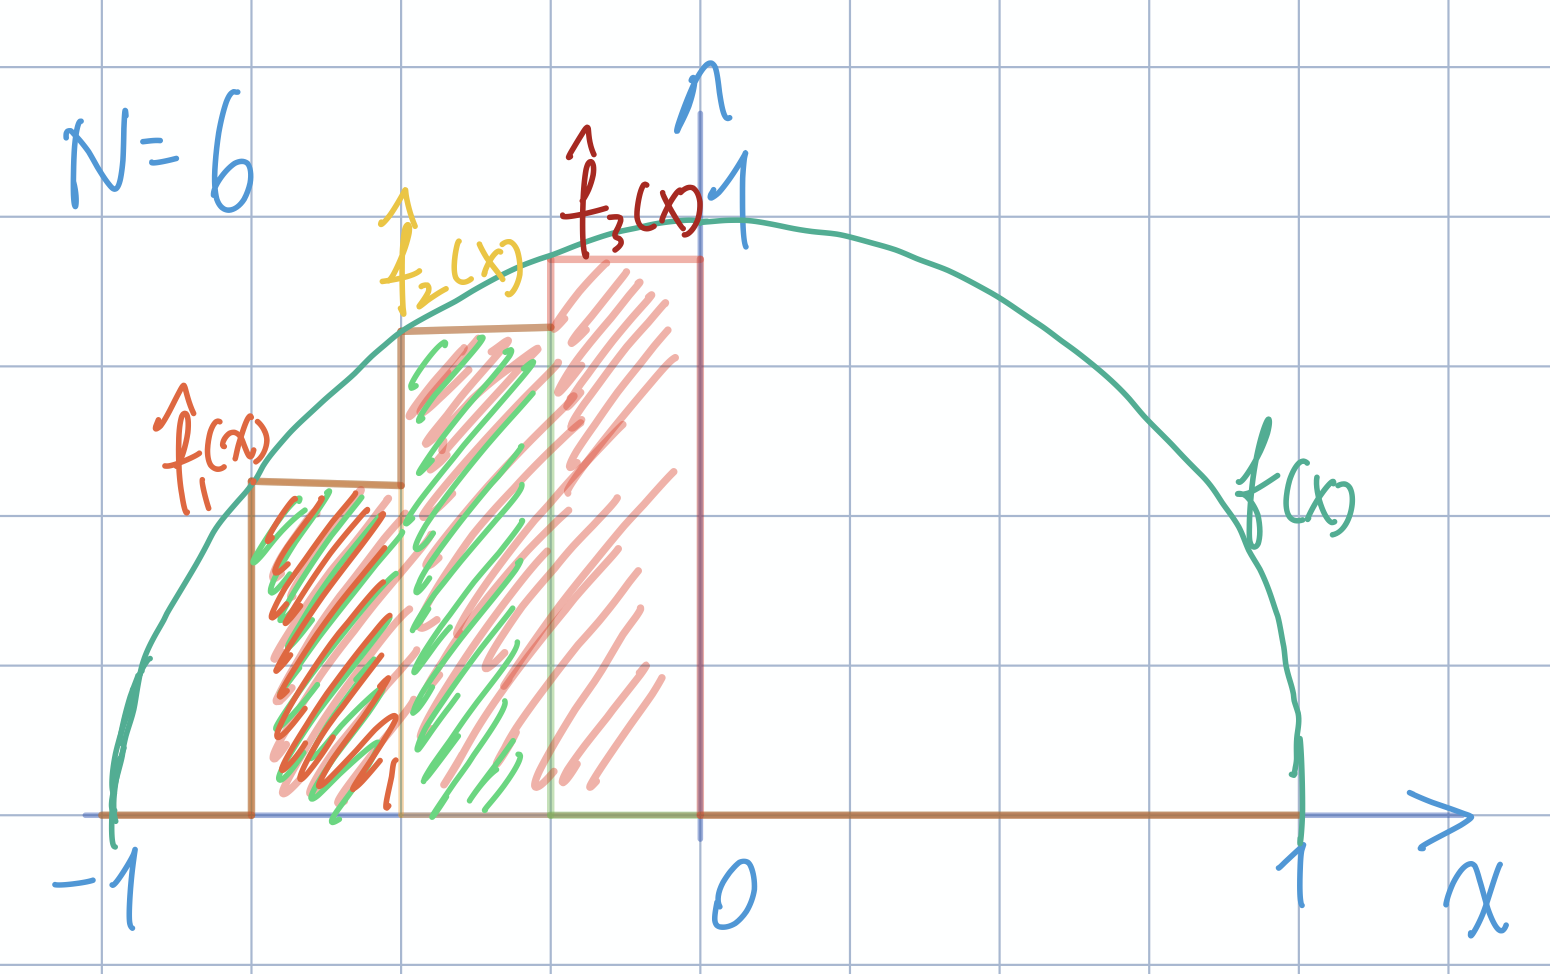
\includegraphics[width=0.7\linewidth]{plot_133.png}
			\caption{Approximated Results for $N=6$}
		\end{figure}
	\end{proof}
	\subsubsection{}
	\begin{proof}[Soln]
		Not required.
	\end{proof}
	
	\section{Backprop}
	\subsection{Computational Graph}
	\subsubsection{}
	\begin{proof}[Soln]
		The computational graph can be drawn as:
		\begin{figure}[H]
			\center
			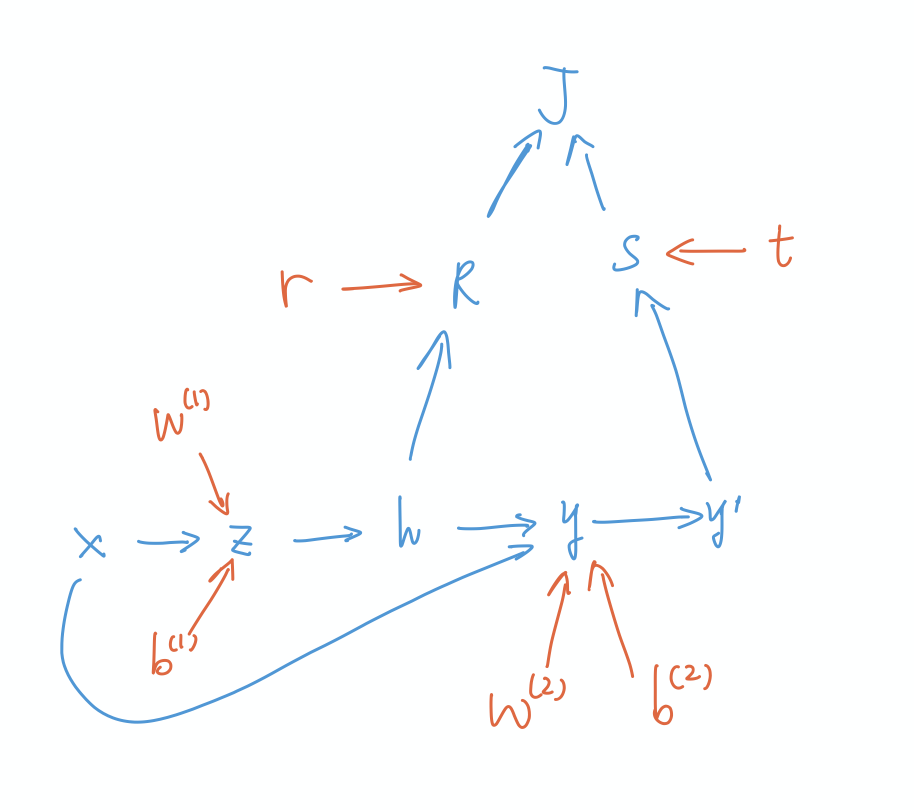
\includegraphics[width=\linewidth]{comp_graph.png}
			\caption{Computational Graph}
		\end{figure}
	\end{proof}
	\subsubsection{}
	\begin{proof}[Soln]
		For individual derivatives:
		\begin{align}
			\overline{\mc{J}} &= \pd{\mc{J}}{\mc{J}} = 1 \\
			\overline{\mc{R}} &= \pd{\mc{J}}{\mc{R}} = \overline{\mc{J}}1 \\
			\overline{\mc{S}} &= \overline{\mc{J}} (-1) \\
			\overline{\textbf{r}} &= \overline{\mc{R}} \pd{\mc{R}}{\textbf{r}} = \overline{\mc{R}} \textbf{h} \\
			\overline{\textbf{y}'} &= \overline{\mc{S}} \pd{\mc{S}}{\textbf{y}'} = \overline{\mc{S}} \textbf{e}_t \\
			\overline{\textbf{y}} &= \overline{\textbf{y}'} \pd{\textbf{y}'}{\textbf{y}} = \overline{\textbf{y}'}\texttt{softmax}'(\textbf{y}) \\
			\overline{\textbf{h}} &= \overline{\mc{R}} \pd{\mc{R}}{\textbf{h}} + \overline{\textbf{y}} \pd{\textbf{y}}{\textbf{h}} = \overline{\mc{R}} \textbf{r} + \overline{\textbf{y}} \textbf{W}^{(2)} \\
			\overline{\textbf{b}^{(2)}} &= \overline{\textbf{y}} 1 \\
			\overline{\textbf{W}^{(2)}} &= \overline{\textbf{y}} \textbf{h} \\
			\overline{\textbf{z}} &= \overline{\textbf{h}} \id{\textbf{z} \geq 0} \\
			\overline{\textbf{W}^{(1)}} &= \overline{\textbf{z}} \textbf{x} \\
			\overline{\textbf{b}^{(1)}} &= \overline{\textbf{z}} 1 \\
			\overline{\textbf{x}} &= \overline{\textbf{z}} \textbf{W}^{(1)} + \overline{\textbf{y}} 1
		\end{align}
%		Put everything together:
%		\begin{align}
%			\overline{\textbf{x}} &= \overline{\textbf{z}} \pd{\textbf{z}}{\textbf{x}}\\
%			&= \overline{\textbf{z}} \textbf{W}^{(1)} \\
%			&= \overline{\textbf{h}} \pd{\textbf{h}}{\textbf{z}} \textbf{W}^{(1)} \\
%			&= \overline{\textbf{h}} \id{\textbf{z} \geq 0} \textbf{W}^{(1)} \\
%			&= \left (
%			\overline{\mc{R}} \pd{\mc{R}}{\textbf{h}}
%			+ \overline{\textbf{y}} \pd{\textbf{y}}{\textbf{h}}
%			\right)
%			\id{\textbf{z} \geq 0} \textbf{W}^{(1)} \\
%			&= \left (
%			\overline{\mc{R}} \textbf{r}^T
%			+ \overline{\textbf{y}} \textbf{W}^{(2)}
%			\right)
%			\id{\textbf{z} \geq 0} \textbf{W}^{(1)} \\
%			&= \left (
%			\textbf{r}^T
%			+ \overline{\textbf{y}'} \pd{\textbf{y}'}{\textbf{y}} \textbf{W}^{(2)}
%			\right)
%			\id{\textbf{z} \geq 0} \textbf{W}^{(1)} \\
%			&= \left (
%			\textbf{r}^T
%			+ \overline{\textbf{y}'} \texttt{softmax}'(\textbf{y}) \textbf{W}^{(2)}
%			\right)
%			\id{\textbf{z} \geq 0} \textbf{W}^{(1)} \\
%			&= \left (
%			\textbf{r}^T
%			+ \overline{\mc{S}} \pd{\mc{S}}{\textbf{y}'} \texttt{softmax}'(\textbf{y}) \textbf{W}^{(2)}
%			\right)
%			\id{\textbf{z} \geq 0} \textbf{W}^{(1)} \\
%			&= \left (
%			\textbf{r}^T
%			+ \textbf{e}_k\ \texttt{softmax}'(\textbf{y}) \textbf{W}^{(2)}
%			\right)
%			\id{\textbf{z} \geq 0} \textbf{W}^{(1)}
%		\end{align}
		where \textbf{e}$_t$ denotes the one-hot vector in $\R^N$ in which the $t^{th}$ element is one.
	\end{proof}
	\subsection{Vector-Jacobean Product (VJPs)}
	\subsubsection{}
	\begin{proof}[Soln]
		\begin{align}
			\textbf{f}(\vex) &:= \vev \vev^T \vex \\
			\implies J = \frac{d}{d\vex} \textbf{f}(\vex) &= \vev \vev^T \\
			\implies J &=
			\left(
			\begin{array}{ccc}
			 1 & 2 & 3 \\
			 2 & 4 & 6 \\
			 3 & 6 & 9 \\
			\end{array}
			\right)
		\end{align}
	\end{proof}
	
	\subsubsection{}
	\begin{proof}[Soln] Time cost: $n^2$. Memory cost: $\frac{(n+1)n}{2}$ (only need to store elements above the diagonal (including the diagonal), because $J$ is symmetric). Therefore, both time and memory cost are $\mc{O}(n^2)$.
	\end{proof}
	\subsubsection{}
	\begin{proof}[Soln]
		\begin{align}
			J^T \vey &= \vev \vev^T \vey \\
			&= \vev (\vev^T \vey) \\
			&= \underbrace{\vev \overbrace{\inner{\vev}{\vey}}^{\tx{step 1}}}_{\tx{step 2}}\quad (\dagger) \\
			\implies \vez & \vev \sum_{i=1}^3 v_i y_i \\
			\implies \vez^T &= 6 \vev^T \\
			\implies \vez^T &= [6, 12, 18]
		\end{align}
		where the inner product operation has time cost $n$ and its output takes memory cost 1. Let $\alpha = \inner{\vev}{\vey} \in \R$, the vector scaler multiplication operation $\vev \alpha$ has time cost $n$ and its output has memory cost $n$. \\
		The overall time cost for ($\dagger$) is therefore $2n$ and memory cost is $n + 1$. \\
		So that both the memory and time costs are in $\mc{O}(n)$.
	\end{proof}

	\section{Linear Regression}
	\subsection{Driving the Gradient}
	\begin{proof}[Soln]
		\begin{align}
			\frac{d}{d\hat{\textbf{w}}} \frac{1}{n} (X \hat{\textbf{w}} - \textbf{t})^2
			&= \frac{d}{d\hat{\textbf{w}}} \frac{1}{n} \norm{X \hat{\textbf{w}} - \textbf{t}}^2_2 \\
			&= \frac{2}{n} (X \hat{\textbf{w}} - \textbf{t})^T X \\
		\implies \nabla_{\textbf{w}} \mc{J} &= \frac{2}{n} X^T(X\hat{\textbf{w}} - \textbf{t})
		\end{align}
	\end{proof}

	\subsection{Under-parameterized Model}
	\subsubsection{}
	\begin{proof}[Soln]
		Assume $d < n$ so that $X^T X$ is invertible. The gradient descent algorithm converges when the gradient equals zero:
		\begin{align}
			\frac{2}{n} (X \hat{\textbf{w}} - \textbf{t})^T X &= 0 \\
			\implies (X \hat{\textbf{w}} - \textbf{t})^T X &= 0 \\
			\implies X^T (X \hat{\textbf{w}} - \textbf{t}) &= 0^T \\
			\implies X^T X \hat{\textbf{w}} - X^T \textbf{t} &= 0^T \\
			\implies X^T X \hat{\textbf{w}} &= X^T \textbf{t} \\
			\implies \hat{\textbf{w}} &= (X^T X)^{-1} X^T \textbf{t}
		\end{align}
	\end{proof}
	\subsubsection{}
	\begin{proof}[Soln]
		Let $\vex \in \R^d$, note that $(X^T X)^{-1}$ is symmetric. Assuming target \textbf{t} is generated by a linear process, then $\textbf{t} = X \textbf{w}^*$. Immediately, $\textbf{t}^T = \textbf{w}^{*T} X^T$.
		\begin{align}
			(\textbf{w}^{*T} \vex  -  \hat{\textbf{w}}^{T} \vex)^2 
			&= (\textbf{w}^{*T} \vex - [(X^T X)^{-1} X^T \textbf{t}]^T \vex)^2 \\
			&= (\textbf{w}^{*T} \vex - \textbf{t}^T X (X^T X)^{-1} \vex)^2 \\
			&= (\textbf{w}^{*T} \vex - \textbf{w}^{*T} X^T X (X^T X)^{-1} \vex)^2 \\
			&= (\textbf{w}^{*T} \vex - \textbf{w}^{*T} \vex)^2 \\
			&= 0
		\end{align}
	\end{proof}
	
	\subsection{Over-parameterized Model: 2D Example}
	\subsubsection{}
	\begin{proof}[Soln]
%		Assume $d > n$ so that $X X^T$ is invertible.
		To minimize the empirical risk minimizer, 
		\begin{align}
			\min_{w_1, w_2} (w_1 x_1 + w_2 x_2 - t_1)^2 \\
			\tx{equivalently, } \min_{w_1, w_2} (2 w_1 + w_2 - 2)^2
		\end{align}
		Any pair of $(w_1, w_2)$ satisfying
		\begin{align}
			2 w_1 + w_2 - 2 = 0\quad (\dagger)
		\end{align}
		attains the minimum level of empirical risk (zero). Equivalently, any $\hat{\textbf{w}}$ on the line
		\begin{align}
			\hat{\textbf{w}} = \begin{pmatrix}
				0 \\ 2
			\end{pmatrix} + t \begin{pmatrix}
				1 \\ -2
			\end{pmatrix} \tx{ for } t \in \R
		\end{align}
		satisfies ($\dagger$). Therefore, there are infinitely many empirical risk minimizers. \\
		Equivalently, the collection of solution is
		\begin{align}
			w_2 = -2 w_1 + 2
		\end{align}
	\end{proof}
	\subsubsection{}
	\begin{proof}[Soln]
		From the fist part of this question we know that
		\begin{align}
			\nabla_{\textbf{w}} \mc{J} 
			&= \frac{2}{n} (X \hat{\textbf{w}} - \textbf{t})^T X \\
			&= \frac{2}{1} \left [
			\begin{pmatrix}2 \\ 1 \end{pmatrix}
			\cdot
			\begin{pmatrix}
			0 \\ 0	
			\end{pmatrix}
			- 2
			\right ]
			\begin{pmatrix}
				2 \\ 1
			\end{pmatrix} \\
			&= \begin{pmatrix}
				-4 \\ -2
			\end{pmatrix}
		\end{align}
		The unit-norm gradient is
		\begin{align}
			\widehat{\nabla_{\textbf{w}}} \mc{J} 
			&= \begin{pmatrix}
				- \frac{2\sqrt{5}}{5} \\
				- \frac{\sqrt{5}}{5}
			\end{pmatrix}
		\end{align}
		The direction (gradient) does not change along the trajectory.
		Ultimately, the gradient descend algorithm converges to 
		\begin{align}
			\hat{\textbf{w}}^*
			&= \left(\frac{4}{5}, \frac{2}{5} \right)
		\end{align}
		\begin{figure}[H]
			\center
			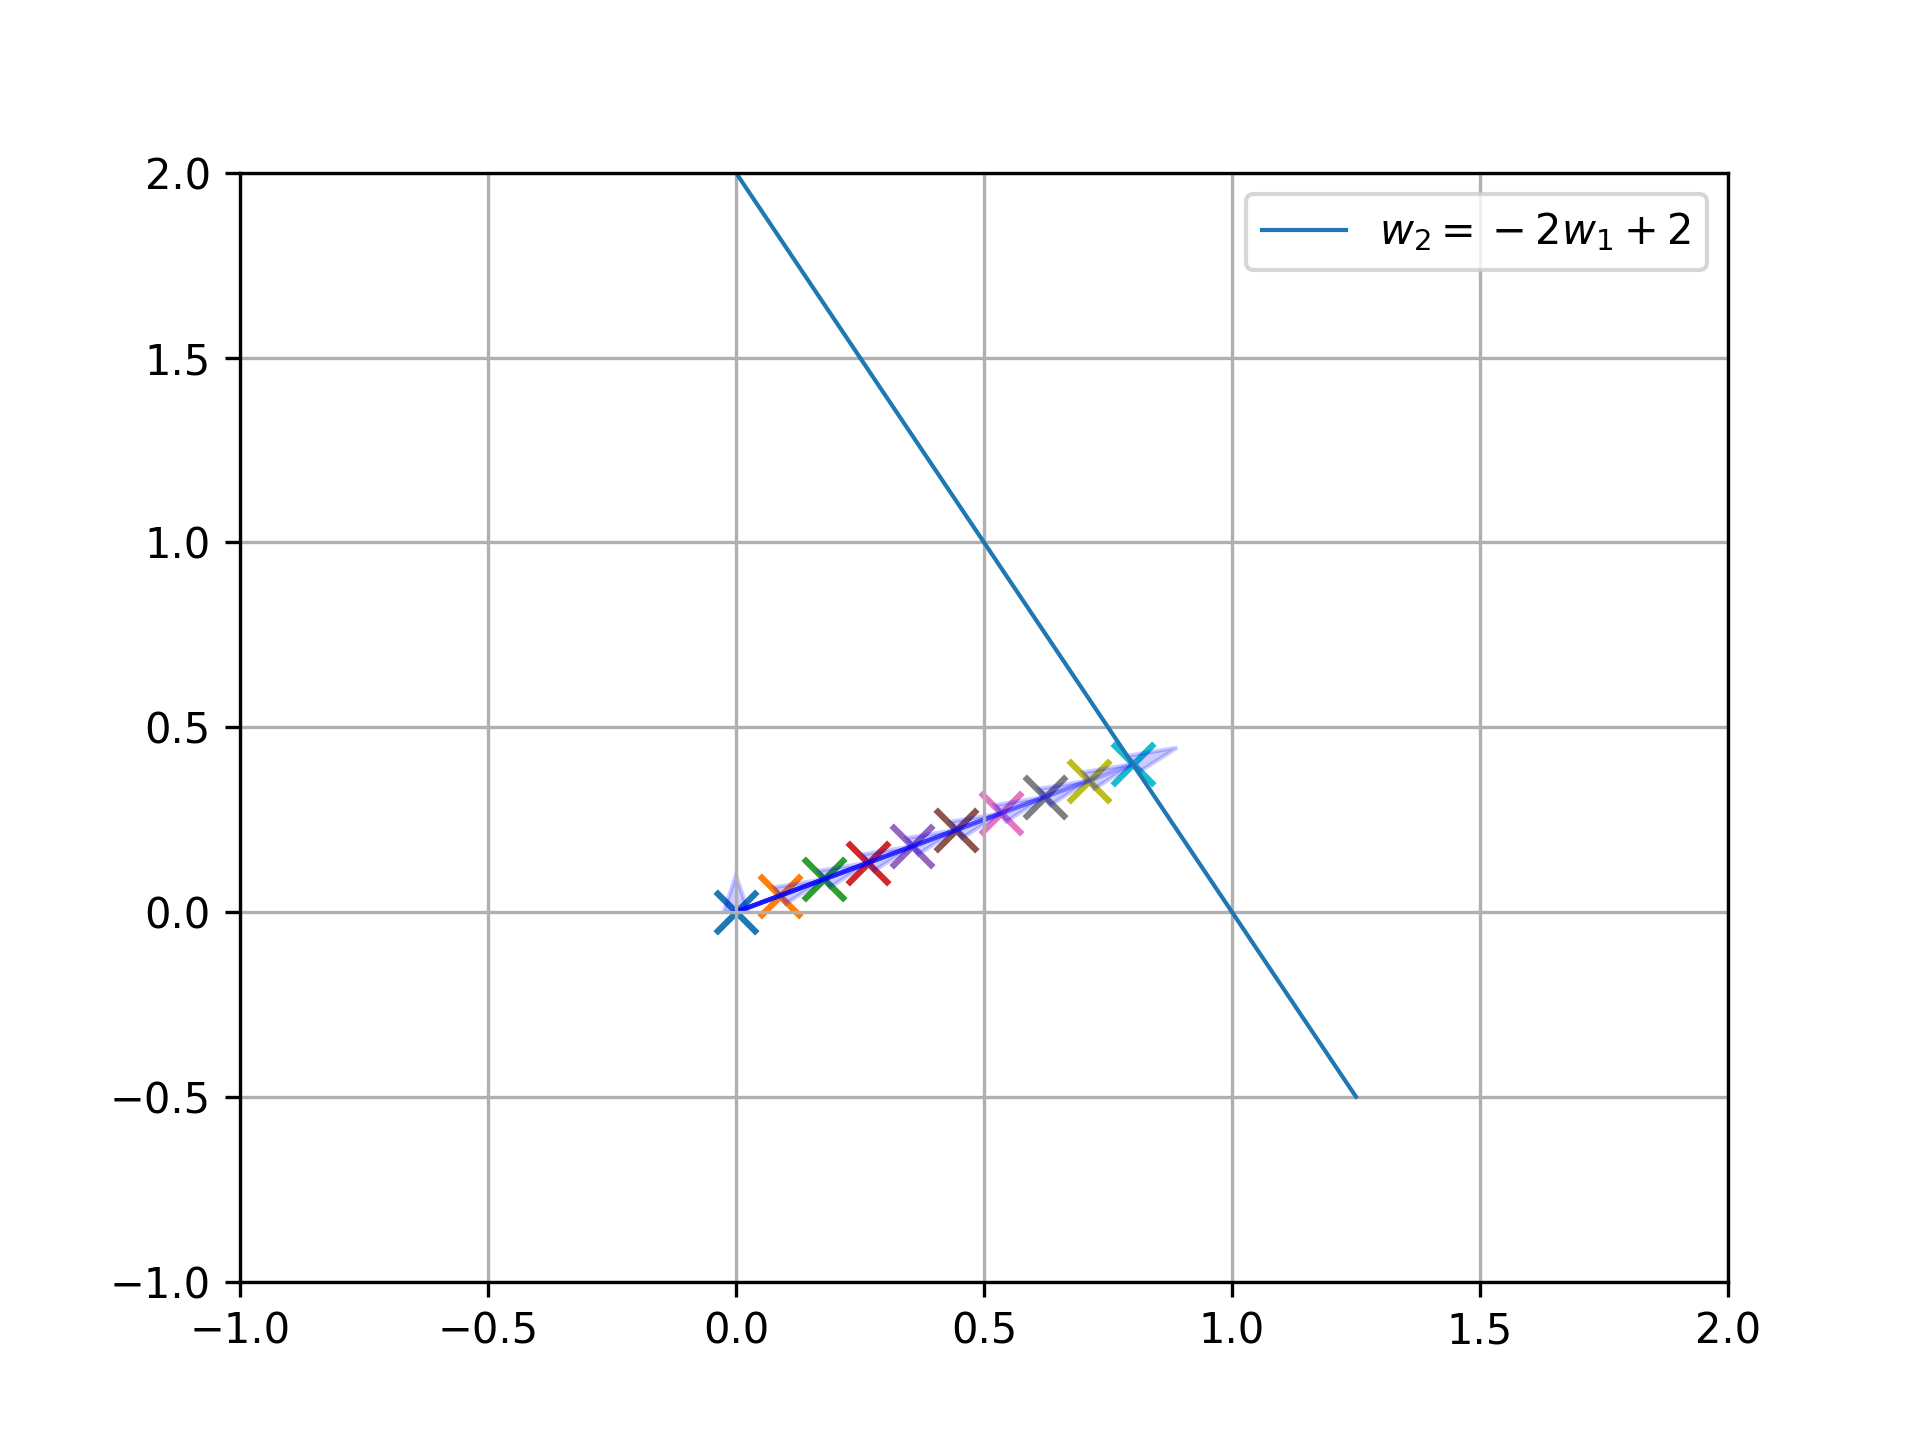
\includegraphics[width=0.7\linewidth]{grad_desc.png}
		\end{figure}
	\end{proof}
	
	\subsubsection{}
	\begin{proof}[Soln]
		Let $\hat{\textbf{w}}^*$ denote the solution found using gradient descent. Note that the line of solution can be written parametrically as
		\begin{align}
			\hat{\textbf{w}}(t) = \begin{pmatrix}
				0 \\ 2
			\end{pmatrix} + t \begin{pmatrix}
				1 \\ -2
			\end{pmatrix}
		\end{align}
		The path of gradient descent starts from $\mc{S} = \textbf{0}$ and the path is perpendicular to the line of solutions $\{\hat{\textbf{w}}(t): t \in \R\}$. By  Pythagorean theorem, we know that the shortest path from a fixed point $x$ to a line $\ell$ is the perpendicular line $x$ and some point $y$ on $\ell$. Meanwhile, $y$ is the point on $\ell$ nearest to $x$. The path of gradient descent is exactly such a shortest path. Therefore, $\hat{\vew}^*$ is the solution nearest to $\textbf{0}$. In another word, $\hat{\vew}$ is solution with smallest Euclidean among all solutions in $\mc{S}$. \\
		Note: this proof is rough and relies on geometric intuition, for a more formal and general proof, please refer to 3.4.2.
	\end{proof}
	
	\subsection{Overparameterized Model: General Case}
	\subsubsection{}
	\begin{proof}
		Note that the solution reached by gradient descent $\vew^*$ can be written as a linear combination of rows of $X$:
		\begin{align}
			X &= \begin{pmatrix}
				x_{11} & \cdots & x_{1d} \\
				\vdots & \ddots & \vdots \\
				x_{n1} & \cdots & x_{nd}
			\end{pmatrix} \\
			\vew^* &= r_1
			\begin{pmatrix}
				x_{11} \\ \vdots \\ x_{1d}
			\end{pmatrix}
			+ \cdots + r_n
			\begin{pmatrix}
				x_{n1} \\ \vdots \\ x_{nd}
			\end{pmatrix} \\
			&= \begin{pmatrix}
				x_{11} & \cdots & x_{1d} \\
				\vdots & \ddots & \vdots \\
				x_{n1} & \cdots & x_{nd}
			\end{pmatrix}^T
			\begin{pmatrix}
				r_1 \\ \vdots \\ r_n
			\end{pmatrix} \\
			&= X^T \textbf{r}
		\end{align}
		The original minimization problem in $\R^d$ (choosing the optimal $\vew \in \R^d$) can be reduced to a minimization problem in $\R^n$ (choosing the optimal $\textbf{r} \in \R^n$). \\
		The gradient descent algorithm converges if and only if zero gradient is encountered, which is characterized by the following condition:
		\begin{align}
			\frac{d}{d\textbf{r}} \frac{1}{n} \norm{X X^T \textbf{r} - \textbf{t}}_2^2 &= 0 \\
			\implies \frac{2}{n} (XX^T \textbf{r} - \textbf{t})^T XX^T &= 0 \\
			\implies XX^T (XX^T \textbf{r} - \textbf{t}) &= 0 \tx{ (take transpose on both sides)} \\
			\implies XX^T XX^T \textbf{r} = XX^T \textbf{t}
		\end{align}
		Because $d > n$, so $rank(XX^T) = n$ and it is invertible. Therefore,
		\begin{align}
			(XX^T)^{-1} XX^T XX^T \textbf{r} &= (XX^T)^{-1} XX^T \textbf{t} \\
			\implies XX^T \textbf{r} &= \textbf{t} \\
			\implies \textbf{r}^* &= (XX^T)^{-1} \textbf{t} \\
			\implies \vew^* &= X^T (XX^T)^{-1} \textbf{t}
		\end{align}
		where the solution is uniquely determined.
	\end{proof}
	
	\subsubsection{}
	\begin{proof}
		Let $\hat{\vew}_1$ be another zero loss weight, then
		\begin{align}
			X \hat{\vew}_1 &= \textbf{t}
		\end{align}
		Immediately,
		\begin{align}
			\hat{\vew}_1^T X^T &= \textbf{t}^T
		\end{align}
		Evaluating
		\begin{align}
			(\hat{\vew} - \hat{\vew}_1)^T \hat{\vew} &= \norm{\hat{\vew}}^2_2 - \hat{\vew}_1^T \hat{\vew} \\
			&= (X^T (XX^T)^{-1} \textbf{t})^T
			(X^T (XX^T)^{-1} \textbf{t})
			- \hat{\vew}_1^T \hat{\vew} \\
			&= \textbf{t}^T (XX^T)^{-1} X (X^T (XX^T)^{-1} \textbf{t})
			- \hat{\vew}_1^T \hat{\vew} \\
			&= \textbf{t}^T (XX^T)^{-1} \textbf{t}
			- \hat{\vew}_1^T X^T (XX^T)^{-1} \textbf{t} \\
			&= \textbf{t}^T (XX^T)^{-1} \textbf{t}
			- \textbf{t}^T (XX^T)^{-1} \textbf{t} \\
			&= 0\quad (\dagger)
		\end{align}
		Because $\hat{\vew}_1$ is chosen arbitrarily, let $\mc{S}$ denote the space of zero-loss weights. ($\dagger$) suggests the optimal solution found by gradient descent $\hat{\vew} \perp \mc{S}$. \\
		Let $\hat{\vew}$ denote the solution found by gradient descent. \\
		Let $\hat{\vew}_\alpha \in \mc{S}$ and $\textbf{v} = \hat{\vew}_\alpha - \hat{\vew}$.
		\begin{align}
			\norm{\hat{\vew}_\alpha}_2^2 &= \norm{\hat{\vew} + \textbf{v}}_2^2 \\
			&= \norm{\hat{\vew}}_2^2 + 2 \textbf{v} \cdot \hat{\vew} + \norm{\textbf{v}}_2^2 \\
			&= \norm{\hat{\vew}}_2^2 + 2 (\hat{\vew}_\alpha - \hat{\vew}) \cdot \hat{\vew} + \norm{\textbf{v}}_2^2 \\
			&= \norm{\hat{\vew}}_2^2 + \norm{\textbf{v}}_2^2 \tx{ by }(\dagger) \\
			&\geq \norm{\hat{\vew}}_2^2
		\end{align}
		Therefore,
		\begin{align}
			\norm{\hat{\vew}_\alpha}_2^2 \geq \norm{\hat{\vew}}_2^2\quad \forall\ \hat{\vew}_\alpha \in \mc{S}
		\end{align}
		And $\hat{\vew}$ is the element with smallest Euclidean norm among all zero-loss solutions in $\mc{S}$.
	\end{proof}
	
	\subsection{Benefit of Overparameterization}
	\subsubsection{}
	\begin{proof}[Soln]
	Fitting function implementation:
	\begin{lstlisting}[language=Python]
def fit_poly(X, d,):
    X_expand = poly_expand(X, d=d, poly_type = poly_type)
    if d > n: # Over-parameterized case
        W = X_expand.T @ np.linalg.inv(X_expand @ X_expand.T) @ t
    else:  # Under parameterized case.
        W = np.linalg.inv(X_expand.T @ X_expand) @ X_expand.T @ t
    return W
	\end{lstlisting}
	Lines fitted and the corresponding losses using both legendre and chebyshev polynomials are presented in figures below. In both experiments, over-parameterization does \textbf{not} always lead to overfitting. In fact, models with a super high degree (say 100) models resulted similar performances compared with low degrees (In the Legendre case, high degree models actually outperformed low degree models).
		\begin{figure}[H]
			\center
			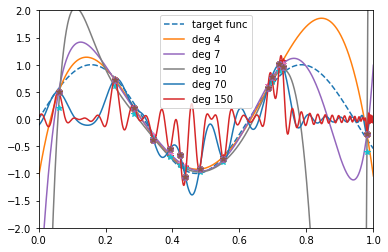
\includegraphics[width=0.45\linewidth]{chebyshev_fit.png}
			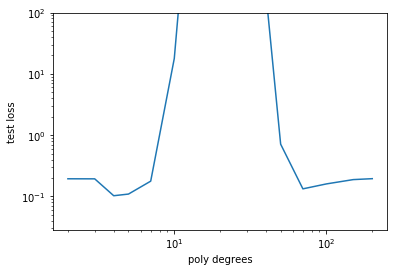
\includegraphics[width=0.45\linewidth]{chebyshev_loss.png}
			\caption{chebyshev results}
		\end{figure}
		\begin{figure}[H]
			\center
			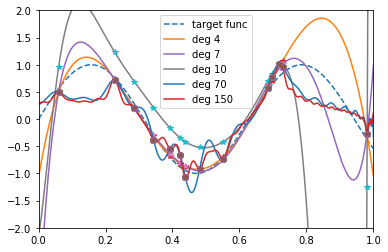
\includegraphics[width=0.45\linewidth]{legendre_fit.png}
			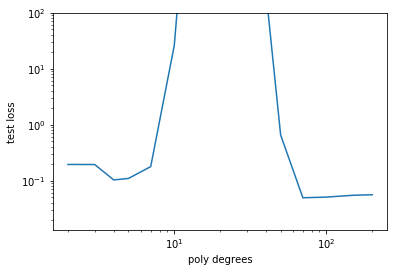
\includegraphics[width=0.45\linewidth]{legendre_loss.png}
			\caption{legendre results}
		\end{figure}
	\end{proof}
	\subsubsection{}
	\begin{proof}[Soln]
		Not required.
	\end{proof}
\end{document}





















